\documentclass[11pt]{article}
\usepackage{graphicx,epstopdf}
\usepackage{mathpazo}
\usepackage{amsmath,amssymb}
\newcommand{\boxeddm}[2]{%
  \[\fbox{%
      %\addtolength{\linewidth}{-2\fboxsep}%
      %\addtolength{\linewidth}{-2\fboxrule}%
      \begin{minipage}{#1\linewidth}%
      $$#2$$%
      \end{minipage}%
    }\]%
}

\begin{document}

\begin{flushright}
Cameron Bracken\\
CVEN 5343\\
PS \#1
\end{flushright}

\begin{enumerate}

%%%%%%%%%%%%%%%%%%%%%%%%
%%%%%%%%%%%%%%%%%%%%%%%%
\item[1. a)] Concentration, $C$, in a 1-D tube is a function of distance along the tube, $x$, time, $t$, the initial mass constituent, $M_0$ and the diffusion coefficient, $D$:

$$f(x,t,M_0,D,C)=0$$

The units: $[x]= L$, $[t]=T$, $[M_0]=M$, $[D] = L^2T^{-1}$, $[C]=ML^{-1}$. 

The matrix system:

$$
\begin{array}{c}
\\L\\T\\M
\end{array}
\begin{array}{c}
	\begin{array}{lllll}
		x & t & M_0 & D & C\\
	\end{array}\\
	\left[
	\begin{array}{ccccc}
		1 & 0 & 0 & 2 & -1\\
		0 & 1 & 0 & -1 & 0\\
		0 & 0 & 1 & 0 & 1\\
	\end{array}
	\right]
\end{array}
\left[
\begin{array}{c}
a_1\\a_2\\a_3\\a_3\\a_4\\a_5
\end{array}
\right]
=0
$$

The system is already in rref form, so read off the solutions

Row 3: $a_3+a_5=0 \longrightarrow$ \fbox{$a_3=-a_5$}

Row 2: $a_2-a_4=0  \longrightarrow$ \fbox{$a_2=a_4$}

Row 1: $a_1+2a_4-a_5=0  \longrightarrow$ \fbox{$a_1=-2a_4+a_5$}

$$
\left[
\begin{array}{c}
a_1\\a_2\\a_3\\a_3\\a_4\\a_5
\end{array}
\right]
= 
\begin{array}{c}
	\begin{array}{c}
		b^I
	\end{array}\\
	\left[
	\begin{array}{c}
		-2\\1\\0\\1\\0
	\end{array}
	\right]
\end{array}
a_4+
\begin{array}{c}
	\begin{array}{c}
		b^{II}
	\end{array}\\
	\left[
	\begin{array}{c}
		-1\\0\\-1\\0\\1
	\end{array}
	\right]
\end{array}
a_5
$$

\boxeddm{.4}{b^I:\,\,\,\,\, x^{-2}tD= \frac{td}{x^2}}
\boxeddm{.4}{b^{II}:\,\,\,\,\, xM_0^{-1}C= \frac{xC}{M_0}}

%%%%%%%%%%%%%%%%%%%%%%%%
%%%%%%%%%%%%%%%%%%%%%%%%
\item[1. b)] Dimensionless concentration is a function of the other dimensionless groups:

$$\frac{xC}{M_0} = f\left(\frac{td}{x^2}\right)$$
\boxeddm{.3}{C = \frac{M_0}{x}f\left(\frac{td}{x^2}\right)}


%%%%%%%%%%%%%%%%%%%%%%%%
%%%%%%%%%%%%%%%%%%%%%%%%
\item[2. a)] Sent via email.


%%%%%%%%%%%%%%%%%%%%%%%%
%%%%%%%%%%%%%%%%%%%%%%%%
\item[2. b)]  The exponential term gives the function its shape (gaussian).  The curve is very tall and skinny when $t$ is small and wide and short when $t$ is large. The term in front of the exponential acts as a scaling factor, that shrinks the profile rapidly at first and then slower as t becomes large. 


%%%%%%%%%%%%%%%%%%%%%%%%
%%%%%%%%%%%%%%%%%%%%%%%%
\item[2. c)]

Integrate over the entire profile, 

$$\int^\infty_{-\infty}C(x,t)\,dx$$.

By symmetry we can integrate only the positive half

\begin{align}
2\int^\infty_{0}C(x,t)\,dx &= 2\int^\infty_{0}\frac{M}{\sqrt{4\pi Dt}}e^{-x^2/4Dt}dx\nonumber\\
& = \frac{M}{\sqrt{\pi Dt}}\int^\infty_{0}e^{-x^2/4Dt}dx
\end{align}

Examine only the integral part for now

\begin{equation}
\int^\infty_{0}e^{-x^2/4Dt}dx
\end{equation}

which is equivalent to 

\begin{equation}
\sqrt{\left(\int^\infty_{0}e^{-x^2/4Dt}dx\right)^2}
\end{equation}

Expanding only the squared term

$$\left(\int^\infty_{0}e^{-x^2/4Dt}dx\right)^2 = \int^\infty_{0}e^{-x^2/4Dt}dx\int^\infty_{0}e^{-x^2/4Dt}dx$$

Change the integration variable and combine the two integrals since both variables are independent

\begin{align}
 \int^\infty_{0}e^{-x^2/4Dt}dx\int^\infty_{0}e^{-y^2/4Dt}dy &= \int^\infty_{0}\int^\infty_{0}e^{-x^2/4Dt}e^{-y^2/4Dt}dxdy\nonumber\\
& = \int^\infty_{0}\int^\infty_{0}e^{-(x^2+y^2)/4Dt}dxdy\nonumber
\end{align}

Change to polar coordinates to continue the integration using the calculus formula:

$$\iint_Rf(x,y)\, dxdy = \iint_{R^*}f(r\cos\theta,r\sin\theta)rdrd\theta$$

In this case $R = \{(x,y) | x\in[0,\infty),y\in[0,\infty)\}$ and $R^* = \{(r,\theta) | r\in[0,\infty),\theta\in[0,\frac{\pi}{2})\}$.  The limits on $\theta$ are because we are doing the integration on half the region for each variable. 

Rewriting the integral in polar coordinates

\begin{align}
 \int^{\frac{\pi}{2}}_{0}\int^\infty_{0}re^{-r^2/4Dt}drd\theta &= \left.\int^{\frac{\pi}{2}}_{0}-2Dte^{-r^2/4Dt}\right|^\infty_0d\theta\nonumber\\
& = -2Dt\int^{\frac{\pi}{2}}_{0}(0-1)d\theta\nonumber\\
& = \pi Dt
\end{align}

Put (4) back into (3) into (1)

$$\frac{M}{\sqrt{\pi Dt}}\sqrt{\pi Dt} = M \,\,\,\,\,\,\square$$


%%%%%%%%%%%%%%%%%%%%%%%%
%%%%%%%%%%%%%%%%%%%%%%%%
\item[2. d)]

\begin{align}
C_0 &= \frac{M}{\sqrt{4\pi Dt}}e^{-x_0^2/4Dt}\nonumber\\
\ln\left(\frac{C_0\sqrt{4\pi Dt}}{M}\right) & = \frac{-x_0^2}{4Dt}\nonumber\\
x_0(t) &= \sqrt{-4Dt\ln\left(\frac{C_0\sqrt{4\pi Dt}}{M}\right)}\nonumber
\end{align}

Choosing a value of 1 for $C_0$, the graph is shown below:

\begin{figure}[htbp] %  figure placement: here, top, bottom, or page
   \centering
   \includegraphics[width=\textwidth]{xvt.eps} 
\end{figure}

$C_0$ must be greater than 0 or else the logarithm will blow up.  The funciton increases at first as the pulse moves outward from it initial position.  The funciton begins decreasing as the profile becomes more attenuated and higher concentrations occur only near the source.  After some amount of time ($\approx$8 in this case), the concentration is lower than $C_0$ everywhere and the function becomes undefined. 

\end{enumerate}



\end{document}  



